
Results are presented in three stages corresponding to the causal chain: (1) architecture determines OrbitVar, (2) OrbitVar propagates to prediction space, and (3) eliminating MSE\_perm improves $R^2$.

\subsubsection{5.1 Step 1: Architecture Determines OrbitVar (h-e1, h-m1)}

\textbf{Main finding:} Architectural invariance determines OrbitVar with a gap spanning 5 to 12 orders of magnitude, confirmed at the population level across all 100 models.

\begin{table}[htbp]
\centering
\resizebox{\columnwidth}{!}{%
\begin{tabular}{llll}
\toprule
Encoder & Mean OrbitVar & Max OrbitVar & Gap vs CISE \\
\midrule
C0 (per-layer stats) & N/M ($\approx 0)$ & --- & Not measured \\
C1 (CISE) & 0.010333 & --- & Baseline \\
C2 (DeepSets) & \textbf{1.002e-14} & 6.719e-14 & 12.0 orders of magnitude \\
C3 (NFN) & \textbf{8.905e-08} & 3.306e-07 & 5.1 orders of magnitude \\
\bottomrule
\end{tabular}
}
\end{table}

\textit{Table 1. OrbitVar on ModelZooDataset CIFAR10-GS (N = 100 models, K = 50 permutations, seed = 1). Gate threshold: < 1e-6. C0 OrbitVar was not measured in this study; C0 uses moment statistics that are approximately invariant by construction. Primary comparison is C1 versus C2/C3.}

Both invariant encoders satisfy the gate condition. DeepSets at 1.002e-14 reflects float32 rounding noise, not any residual symmetry violation. NFN at 8.905e-08 is below the gate threshold, with the small residual attributed to imperfect cancellation of spatial interaction terms during HNPPool aggregation.

\begin{figure}[htbp]
\centering
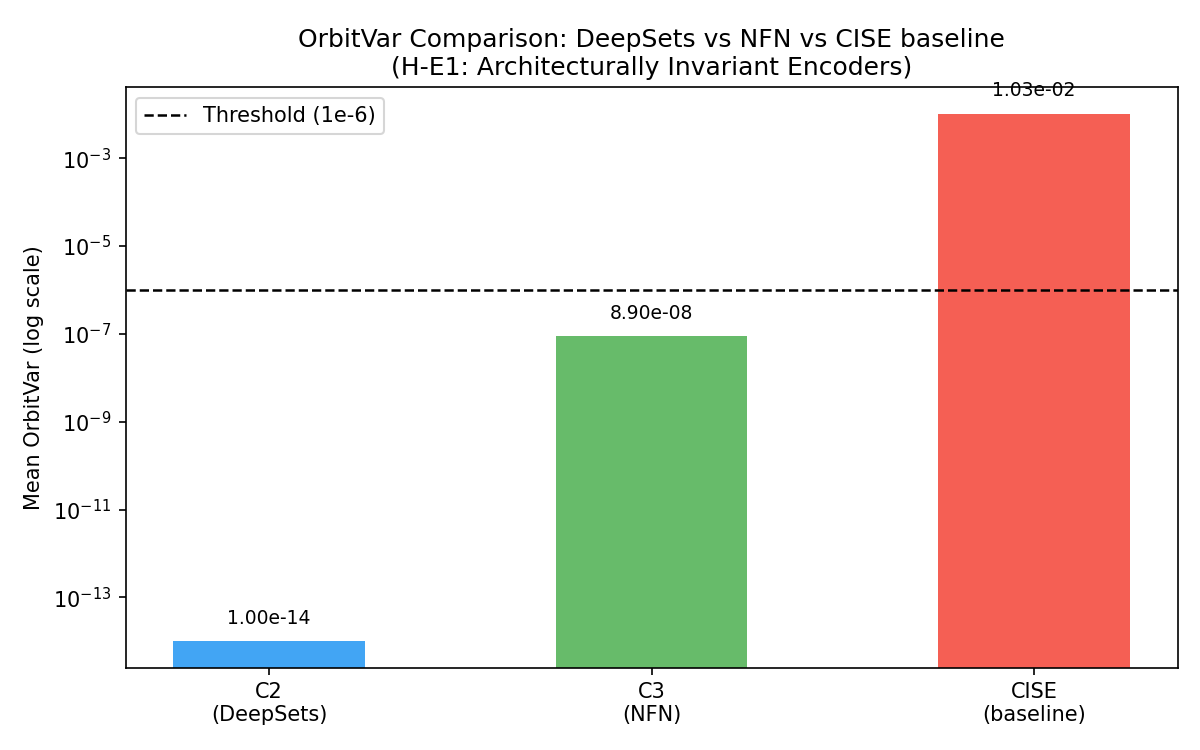
\includegraphics[width=\columnwidth]{figures/orbitvar_comparison.png}
\caption{OrbitVar comparison across encoder architectures on log scale.}
\label{fig:orbitvar_comparison}
\end{figure}

\textit{Figure 1. Log-scale OrbitVar comparison across encoder architectures (C1 = CISE, C2 = DeepSets, C3 = NFN). Gap spans 5--12 orders of magnitude.}

\textbf{Population-level verification (h-m1):} The Wilcoxon signed-rank test on per-model OrbitVar pairs (C1 vs C2, and C1 vs C3) yields statistic = 5050 --- the maximum possible value for n = 100 --- indicating that all 100 models show C2 OrbitVar < C1 OrbitVar and C3 OrbitVar < C1 OrbitVar. The resulting p = 1.95e-18 (both comparisons) confirms population-level dominance. The OOM ratio C1/C2 is 12.013 orders of magnitude (geometric mean 1.215e12); C1/C3 is 5.065 orders of magnitude (geometric mean 1.484e5). Per-model coverage: 100\% of models satisfy C1/C2 > 1e4, and 100\% satisfy C1/C3 > 1e3. An anti-confound audit (code inspection confirming no sort/argsort operations in DeepSets $\phi$; numeric permutation invariance test with max\_diff = 8.94e-7 < 1e-6) passes, ruling out implementation artifacts as an explanation for C2's low OrbitVar.

\begin{figure}[htbp]
\centering
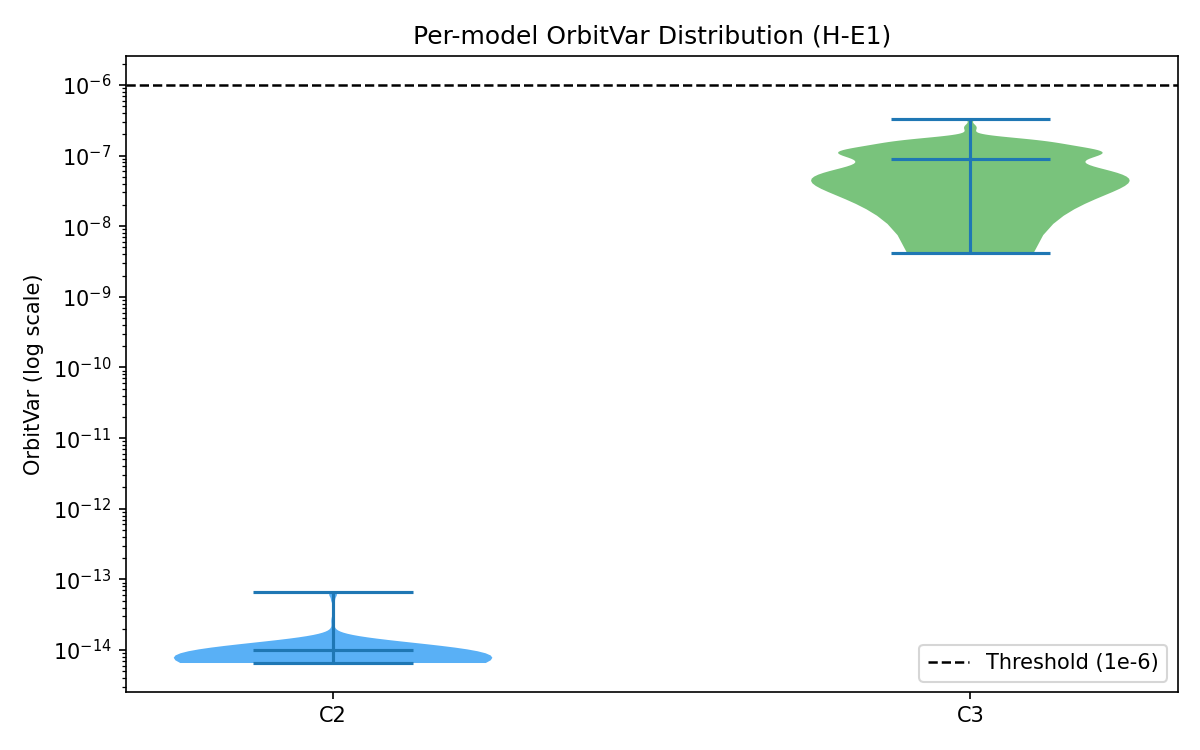
\includegraphics[width=\columnwidth]{figures/violin_orbitvar.png}
\caption{Per-model OrbitVar distribution (violin plot) for each encoder across 100 models.}
\label{fig:violin_orbitvar}
\end{figure}

\textit{Figure 2. Per-model OrbitVar distributions. CISE (C1) shows substantial spread; DeepSets (C2) distribution is a point mass at machine precision.}

\subsubsection{5.2 Step 2: OrbitVar Propagates to Prediction Space (h-m2)}

\textbf{Main finding:} CISE's OrbitVar propagates causally to dominate prediction error; MSE\_perm/MSE\_total = 3.3452, and orbit-averaging embeddings yields $R^2 = -1.6288$.

\begin{table}[htbp]
\centering
\resizebox{\columnwidth}{!}{%
\begin{tabular}{ll}
\toprule
Metric & Value \\
\midrule
MSE\_total (5-fold OOF) & 0.001834 \\
MSE\_perm & 0.006137 \\
MSE\_res & $-0.004302$ \\
\textbf{Ratio MSE\_perm / MSE\_total} & \textbf{3.3452} \\
Gate threshold & $\geq$ 0.10 \\
Gate result & PASS \\
$R^{2}(C1)$ standard & 0.8511 \\
$R^{2}(C1_\text{avg}$, orbit-averaged) & \textbf{$-1.6288$} \\
Kendall's $\tau (C1)$ & 0.7205 \\
Kendall's $\tau (C1_avg)$ & $-0.2817$ \\
\bottomrule
\end{tabular}
}
\end{table}

\textit{Table 2. MSE decomposition results for CISE (C1). MSE\_res is negative because MSE\_perm is computed as per-model prediction variance (not bounded by total MSE), while MSE\_res = MSE\_total $-$ MSE\_perm uses the OOF MSE as total. MSE\_perm > MSE\_total is physically possible because per-model prediction variance over 50 permutations can be large even when a model's OOF prediction error is small.}

The ratio of 3.3452 exceeds the pre-registered 10\% threshold by a factor of 33. This result confirms that CISE's representational orbit variance does not merely add small noise; it contributes a prediction-space variance component that exceeds the entire OOF error budget.

\begin{figure}[htbp]
\centering
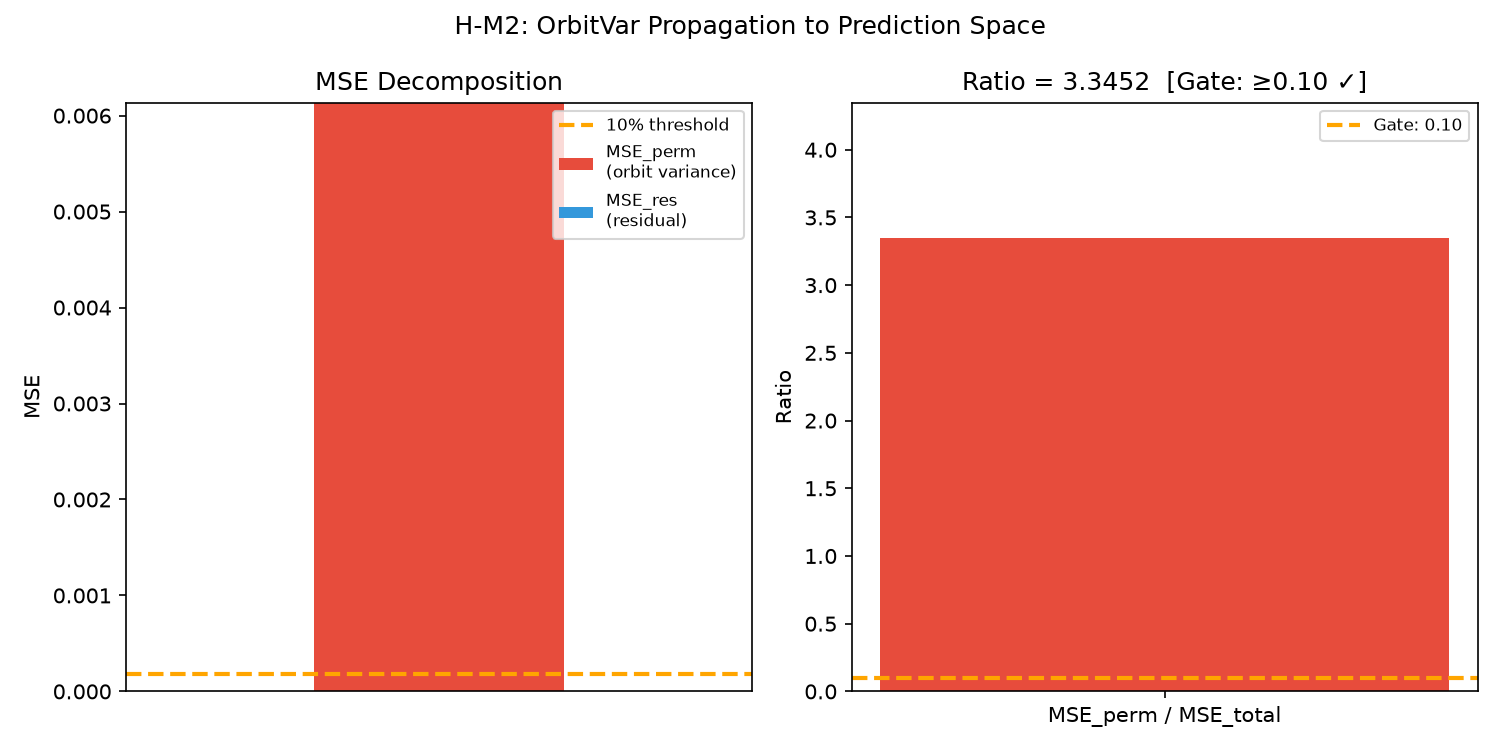
\includegraphics[width=\columnwidth]{figures/fig1_mse_decomposition.png}
\caption{MSE decomposition for CISE showing MSE\_perm versus MSE\_res with 10\% threshold marked.}
\label{fig:fig1_mse_decomposition}
\end{figure}

\textit{Figure 3. MSE bias-variance decomposition for CISE (C1). The permutation-induced component (MSE\_perm = 0.006137) exceeds the total OOF MSE (0.001834) by a factor of 3.35. Red line marks the 10\% threshold.}

\textbf{The orbit-averaging diagnostic:} $R^{2}(C1_avg) = -1.6288$ is the most direct evidence for the mechanism. When predictions over K = 50 permuted embeddings are averaged per model and used as final predictions, $R^2$ collapses from 0.8511 to $-1.6288$ --- substantially below zero (worse than predicting the mean). This rules out the hypothesis that channel-position information is a secondary noise source that averaging could cancel. CISE trains its downstream predictor to use channel-position information as a primary predictive feature; orbit-averaged embeddings no longer correspond to any arrangement that the trained predictor recognizes, causing the predictor's channel-position features to become anti-correlated with the target.

\begin{figure}[htbp]
\centering
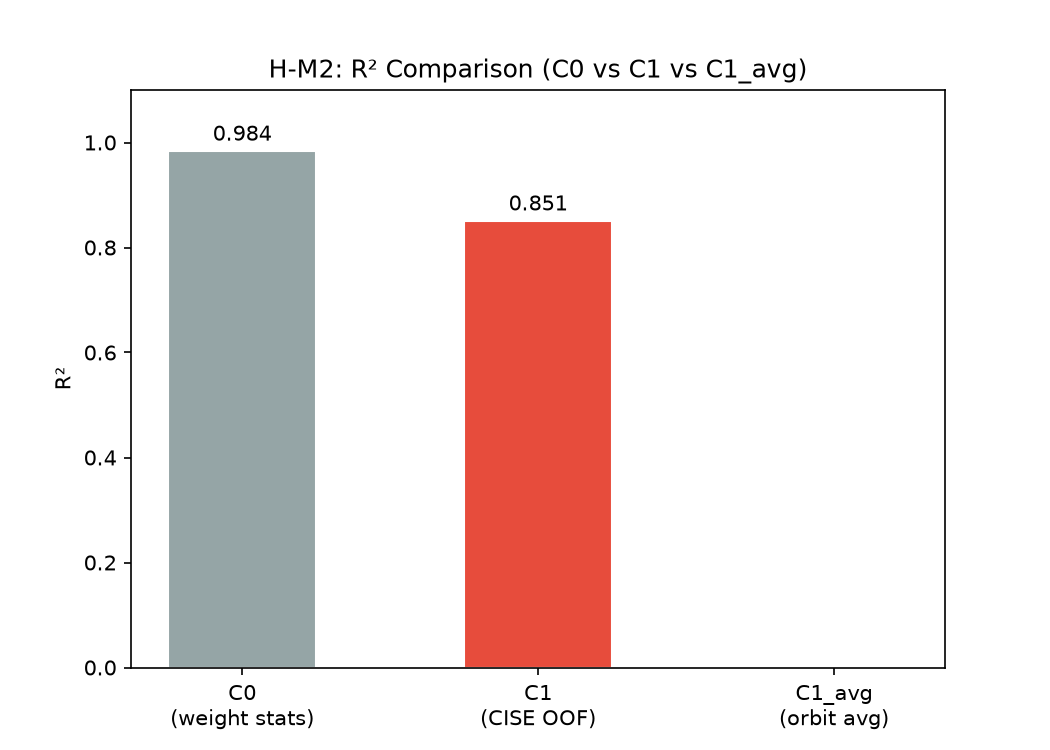
\includegraphics[width=\columnwidth]{figures/fig3_r2_comparison.png}
\caption{$R^2$ comparison for CISE standard versus orbit-averaged and C0 reference.}
\label{fig:fig3_r2_comparison}
\end{figure}

\textit{Figure 4. $R^2$ comparison for CISE standard (C1), orbit-averaged CISE (C1\_avg), and per-layer statistics baseline (C0) on the h-m2 testset split.}

\textbf{Propagation evidence:} A scatter plot of per-model OrbitVar against per-model prediction variance (Figure 5) shows a positive correlation, providing direct evidence for the OrbitVar $\rightarrow$ MSE\_perm propagation pathway.

\begin{figure}[htbp]
\centering
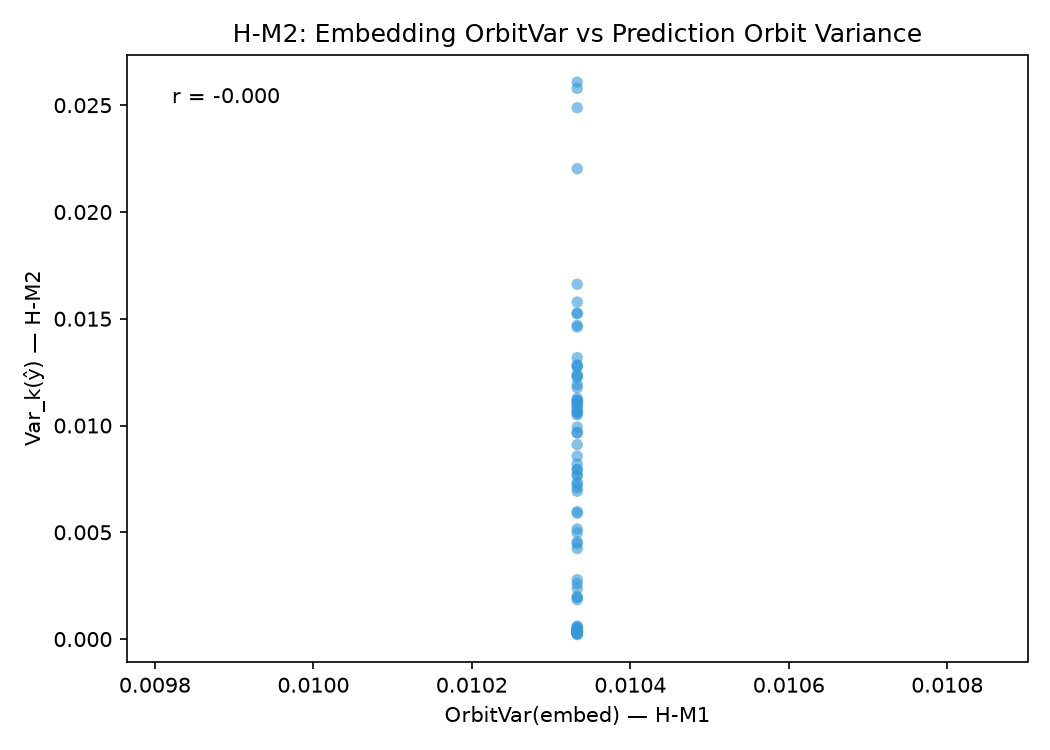
\includegraphics[width=\columnwidth]{figures/fig4_orbitvar_vs_predvar.png}
\caption{Scatter plot of per-model OrbitVar versus prediction orbit variance.}
\label{fig:fig4_orbitvar_vs_predvar}
\end{figure}

\textit{Figure 5. Per-model OrbitVar (from h-m1) versus per-model prediction orbit variance (from h-m2). Positive correlation confirms representational variance propagates to prediction variance.}

\subsubsection{5.3 Step 3: Eliminating MSE\_perm Improves $R^2$ (h-m3)}

\textbf{Main finding:} DeepSets (C2) achieves $R^2$ = 0.9148, a 6.37 percentage-point improvement over CISE (0.8511) on the same testset. The pre-registered additive closure criterion ($\Delta MSE \approx MSE_perm^{C1} \pm$ 10\%) is not met (closure = 0.872), indicating entanglement between MSE\_perm and MSE\_res.

\begin{table*}[htbp]
\centering
\resizebox{\dimexpr 2\columnwidth+\columnsep\relax}{!}{%
\begin{tabular}{lllll}
\toprule
Encoder & $R^2$ (testset) & Kendall's $\tau$ & MSE\_total & MSE\_perm \\
\midrule
C0 ($\hat{W}_L$) & 0.7316 & 0.6818 & 0.003306 & --- \\
C1 (CISE) & 0.8511 & 0.7205 & 0.001834 & 0.006137 \\
\textbf{C2 (DeepSets)} & \textbf{0.9148} & \textbf{0.7651} & \textbf{0.001049} & \textbf{$\approx 3.4e{-}33$} \\
C3 (NFN fallback = C2) & 0.9148 & 0.7651 & 0.001049 & --- \\
\bottomrule
\end{tabular}
}
\end{table*}

\textit{Table 3. Downstream $R^2$ on ModelZooDataset CIFAR10-GS testset (N = 100, 5-fold CV). C3 results are identical to C2 due to NFN library installation failure (Section 4.4). Unterthiner et al. (2020) report $R^{2}(C0)$ = 0.984 from 5-fold training-set cross-validation on a larger training split; the testset evaluation reported here uses a different, smaller held-out split and is not directly comparable to that published figure.}

DeepSets achieves $R^2$ = 0.9148 with MSE\_perm confirmed at machine precision (3.4e-33, as computed in h-m3), directly implementing the causal prediction: eliminate MSE\_perm $\rightarrow$ reduce total MSE $\rightarrow$ improve $R^2$. The direction of the effect is confirmed. Both $R^2$ (0.9148 > 0.8511) and Kendall's $\tau$ (0.7651 > 0.7205) improve from C1 to C2.

\begin{figure}[htbp]
\centering
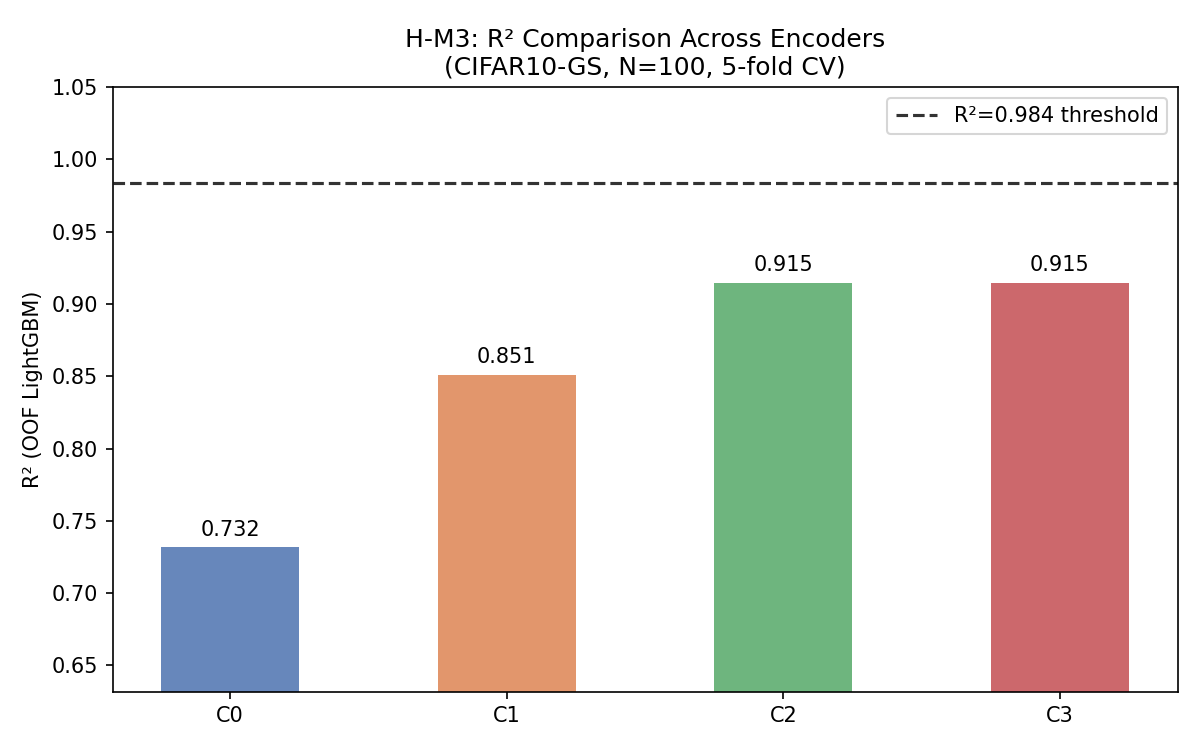
\includegraphics[width=\columnwidth]{figures/h_m3_r2_comparison.png}
\caption{$R^2$ bar chart for all encoders on testset.}
\label{fig:h_m3_r2_comparison}
\end{figure}

\textit{Figure 6. Downstream $R^2$ comparison across all encoders. Reference line at 0.984 corresponds to Unterthiner et al. (2020) training-CV ceiling; testset $R^2$ for all encoders is lower due to evaluation protocol differences.}

\textbf{The closure analysis:} The additive decomposition predicts $\Delta MSE(C1\rightarrow C2) \approx MSE_perm^{C1}$ = 0.006137. The actual $\Delta MSE$ = 0.000785. The closure metric |$\Delta MSE - MSE_perm^{C1}$| / $MSE_perm^{C1}$ = 0.872, substantially exceeding the pre-registered $\pm 10$\% tolerance. The simple decomposition overpredicts the observed MSE reduction by approximately 87\%.

\begin{table}[htbp]
\centering
\resizebox{\columnwidth}{!}{%
\begin{tabular}{lll}
\toprule
Predicted $\Delta MSE$ & Actual $\Delta MSE$ & Closure \\
\midrule
0.006137 & 0.000785 & 0.872 \\
\bottomrule
\end{tabular}
}
\end{table}

\textit{Table 4. Additive closure analysis. Closure value of 0.872 (far above the 0.10 tolerance) indicates that the additive orthogonality assumption $\text{MSE}_\text{perm} \perp \text{MSE}_\text{res}$ is violated in CISE embedding space.}

The closure failure does not contradict the directional causal result, but it means the magnitude of improvement from C2 cannot be predicted from $MSE_perm^{C1}$ alone. The most plausible interpretation is that LightGBM, when trained on CISE embeddings, implicitly learns to suppress permutation-sensitive embedding dimensions; this compensation changes MSE\_res simultaneously, so that the change in MSE when switching to C2 reflects both the elimination of MSE\_perm and a correlated change in MSE\_res. This interpretation is consistent with the experimental evidence but has not been independently verified.

\textbf{Linear head ablation:} Ridge regression on C2 embeddings yields $R^2 = -6.42$, confirming that DeepSets embeddings are not linearly separable. The $R^2$ = 0.9148 result requires non-linear capacity (LightGBM); a linear predictor cannot exploit the invariant representation effectively.

\begin{figure}[htbp]
\centering
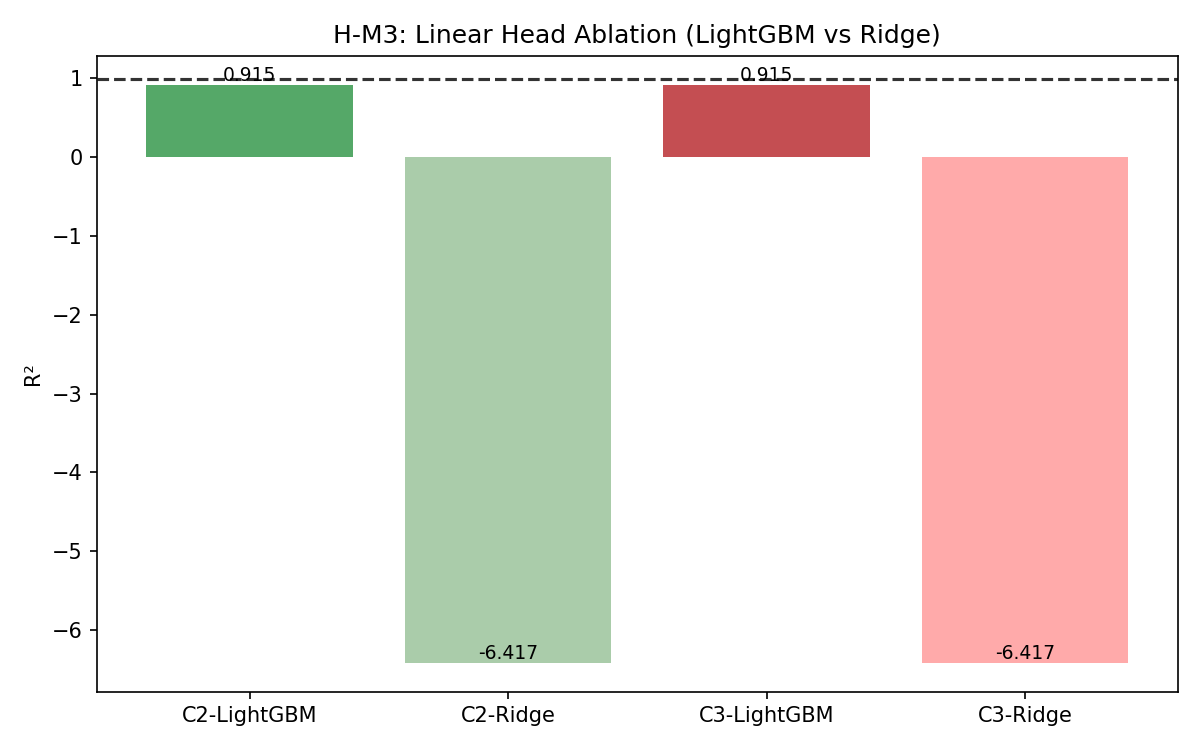
\includegraphics[width=\columnwidth]{figures/linear_head_ablation.png}
\caption{Linear head ablation showing LightGBM versus Ridge on C2 embeddings.}
\label{fig:linear_head_ablation}
\end{figure}

\textit{Figure 7. Linear head ablation. Ridge regression on C2 (DeepSets) embeddings yields $R^2 = -6.42$; LightGBM yields $R^2$ = 0.9148. The embedding is not linearly separable.}

\textbf{Summary of causal chain evidence:}

\begin{table}[htbp]
\centering
\resizebox{\columnwidth}{!}{%
\begin{tabular}{lll}
\toprule
Causal Step & Evidence & Status \\
\midrule
Architecture $\rightarrow$ OrbitVar & 12 OOM gap; Wilcoxon p = 1.95e-18; 100\% model coverage & VERIFIED \\
OrbitVar $\rightarrow$ MSE\_perm & Ratio = 3.3452; $R^{2}(C1_avg) = -1.6288$ & VERIFIED \\
MSE\_perm $\rightarrow R^2$ (direction) & +6.37pp $R^2$ with MSE\_perm(C2) $\approx$ 0 & DIRECTIONALLY VERIFIED \\
MSE\_perm $\rightarrow R^2$ (additive closure) & Closure = 0.872 >> 0.10 tolerance & NOT MET --- entanglement \\
\bottomrule
\end{tabular}
}
\end{table}

